% !TeX root = ../../tesi.tex

\section{I limiti degli assistenti conversazionali testuali}
\label{sec:limiti-assistenti}

Molti negozi \emph{online} offrono ai clienti un \gloss{chatbot}{\emph{chatbot}}, un programma che
conversa con l’utente in linguaggio naturale. Di solito compare come
\gloss{widget}{\emph{widget}}, un riquadro sovrapposto alle pagine del negozio che il cliente apre
con un pulsante. Questi assistenti rispondono quasi sempre con solo testo. Il testo è adatto alle
domande frequenti, ma è poco efficace quando il cliente deve confrontare prodotti, scegliere una
taglia o controllare un ordine, cioè nelle operazioni che le pagine di un negozio risolvono con
immagini, prezzi, selettori e pulsanti. Un assistente che descrive a parole tre prodotti costringe
il cliente ad abbandonare la conversazione per vederli, e per il commerciante questo si traduce in
conversazioni che non si concludono con un acquisto. La \figref{fig:confronto} mette a confronto le
due risposte alla stessa richiesta.

\begin{figure}[htbp]
	\centering
	\setstretch{1}
	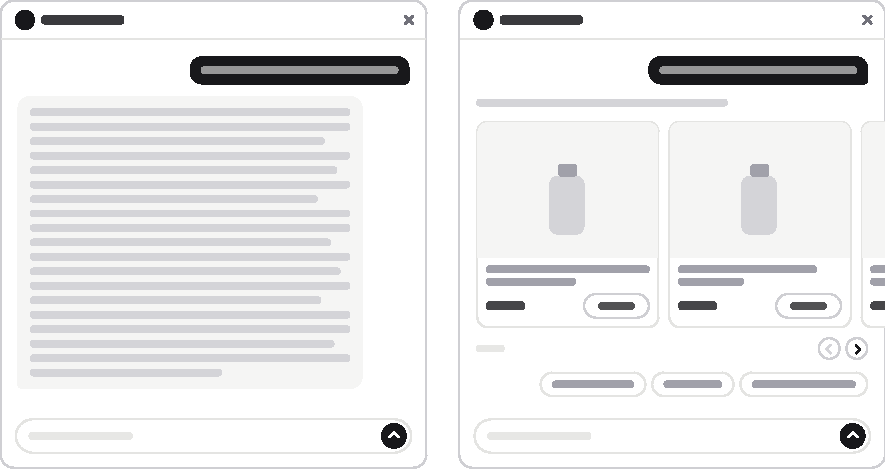
\includegraphics[width=\textwidth]{figure/02-ragioni/confronto.pdf}
	\caption[Confronto tra un assistente testuale e ChatCart]{\emph{Mockup} della risposta alla
	stessa richiesta di un assistente testuale, a sinistra, e di ChatCart, a destra.}
	\label{fig:confronto}
\end{figure}

Il potenziale di un assistente efficace è misurabile. Uno studio sperimentale condotto tra il 2023
e il 2024 su una delle maggiori piattaforme internazionali di commercio
elettronico\textsuperscript{\ref{rif:studio-genai}} ha confrontato sette applicazioni dell’IA
generativa, ciascuna con un gruppo di clienti che la usava e un gruppo di controllo. L’effetto
maggiore è quello dell’assistente che risponde alle domande dei clienti prima dell’acquisto, che ha
aumentato le vendite del 16,3\%. L’aumento deriva da un numero maggiore di clienti che acquistano,
mentre il valore medio del carrello resta invariato. I clienti che traggono più vantaggio
dall’assistente sono quelli che conoscono meno la piattaforma.

Le soluzioni disponibili sul mercato appartengono a cinque tipi, e ciascuno lascia scoperta una
parte del problema:

\begin{itemize}
	\item \textbf{Gli assistenti generici per l’assistenza clienti} risolvono richieste di supporto
	su più canali a partire dai documenti dell’azienda. Conoscono poco il catalogo e rispondono con
	testo, quindi sono adatti alla gestione di un reso più che alla scelta di un prodotto.
	\item \textbf{Gli assistenti alla vendita preconfezionati} si installano nel negozio e
	consigliano prodotti. L’interfaccia, il modello e il comportamento sono decisi dal fornitore e
	restano uguali per tutti i negozi che li adottano.
	\item \textbf{Sidekick}\textsuperscript{\ref{rif:sidekick}}, l’assistente che Shopify integra nel
	pannello di amministrazione, supporta il commerciante nella gestione del negozio e non si
	rivolge a chi acquista.
	\item \textbf{Il \emph{server} MCP del negozio}\textsuperscript{\ref{rif:storefront-mcp}}, che
	Shopify attiva per ogni negozio, espone agli agenti la ricerca nel catalogo, il carrello e le
	condizioni di vendita. È un componente destinato a chi sviluppa un agente, perché fornisce dati
	e operazioni senza un’interfaccia, e la sua ricerca è la stessa per ogni catalogo.
	\item \textbf{\gloss{ucp}{UCP}}\textsuperscript{\ref{rif:ucp}}, uno standard aperto che Shopify
	e Google hanno pubblicato nel gennaio 2026, permette a un agente di scoprire che cosa offre un
	negozio e di completare un acquisto. È pensato per gli assistenti di terze parti, per cui la
	conversazione avviene fuori dal negozio, in un’interfaccia che il marchio non controlla.
\end{itemize}

Nessuna di queste soluzioni soddisfa insieme i tre requisiti a cui i clienti di Halue attribuiscono
più valore, cioè l’identità visiva del marchio, i dati specifici del suo catalogo e un’esperienza
d’acquisto che si svolge interamente nel negozio. Un prodotto preconfezionato deve adattarsi a
tutti i commercianti, e per questo lascia poco spazio alla personalizzazione. Halue costruisce
soluzioni per il singolo cliente, perciò ha scelto di esplorare un assistente su misura basato su
un’\gloss{interfaccia-generativa}{interfaccia generativa}, in cui l’agente risponde con testo
oppure sceglie un componente da una libreria predefinita, come una scheda prodotto, e lo popola in
tempo reale con i dati del negozio. Il marchio conserva il controllo sull’aspetto dei componenti,
e il modello decide soltanto quale mostrare e con quali dati.
